\begin{figure}[!htb]
  \centering
  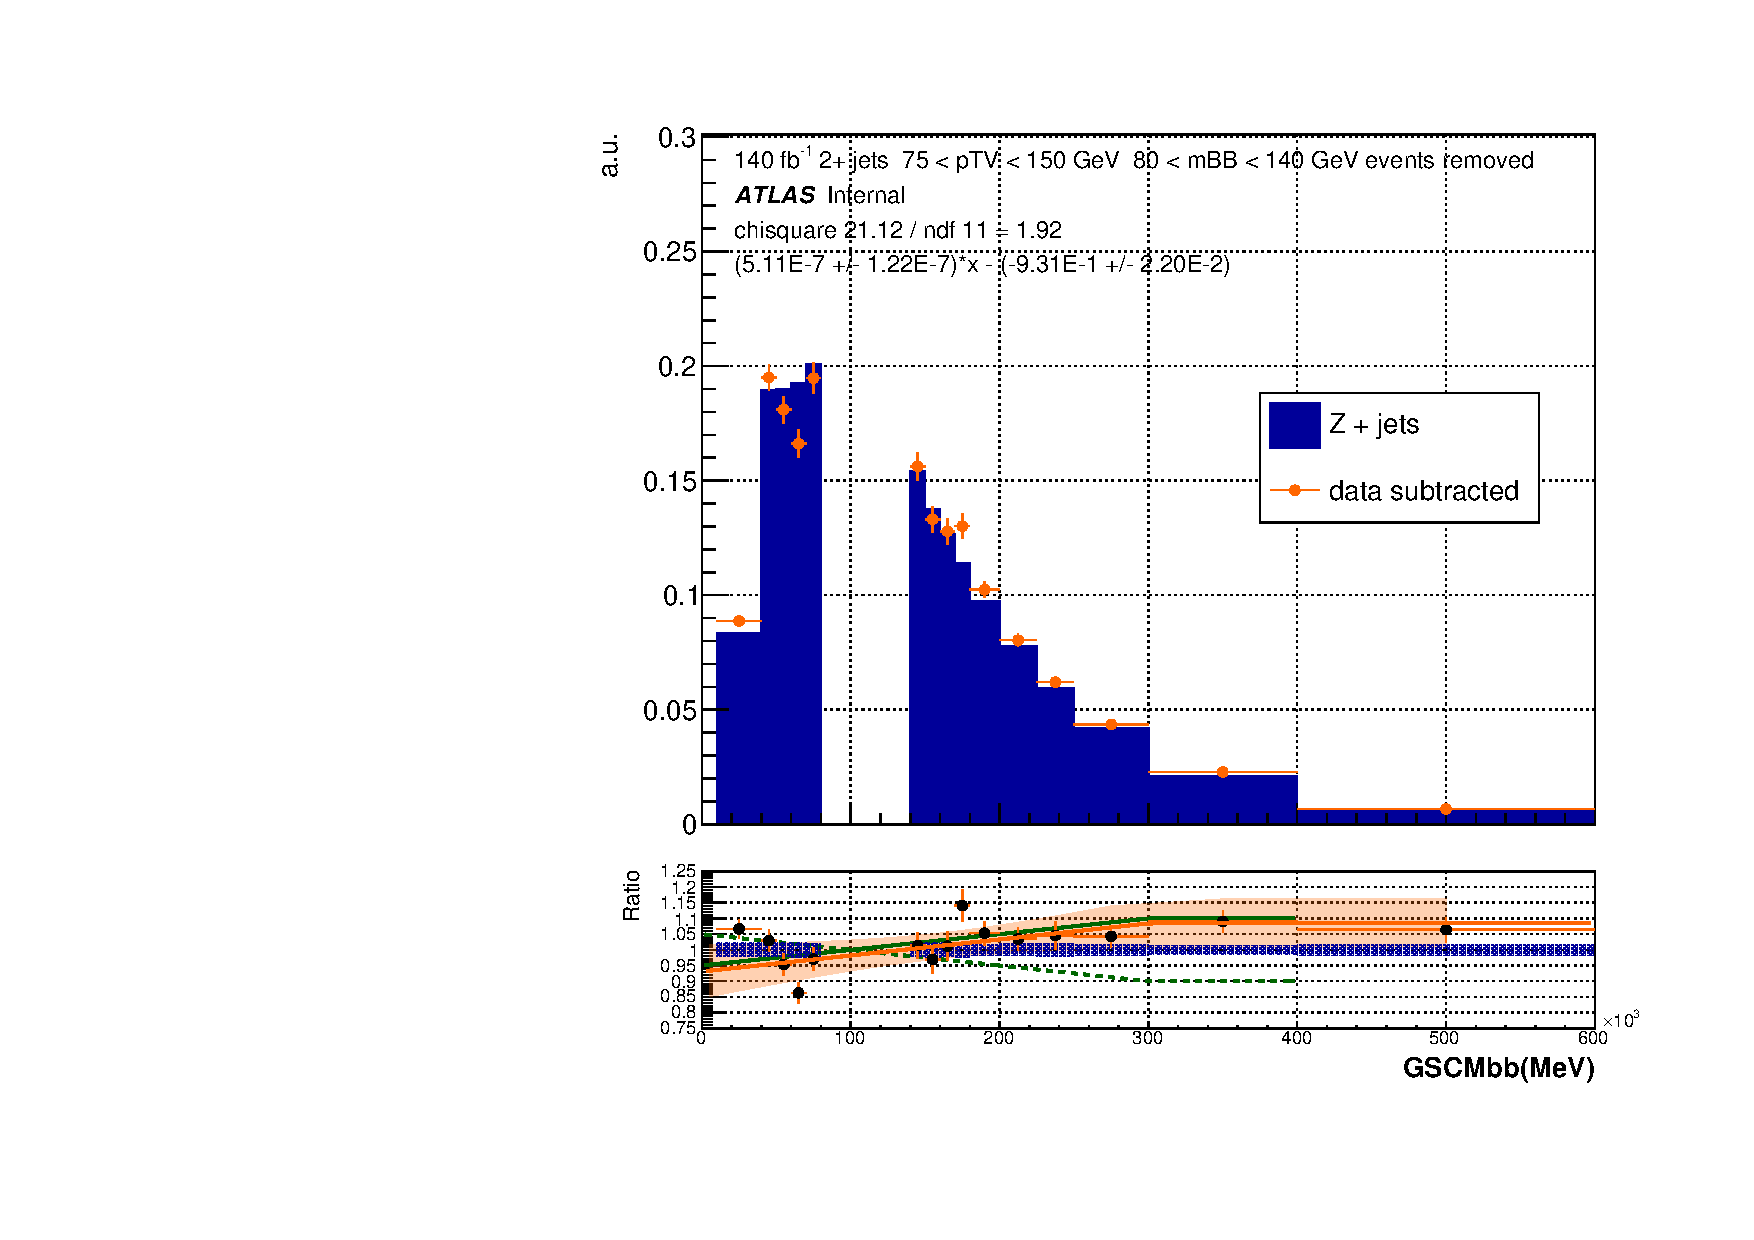
\includegraphics[width=0.49\textwidth]{Zjets-shapes/two_plus_jet_low_blind_ttbardd/two_plus_jet_low_blind_ttbardd_GSCMbb}
  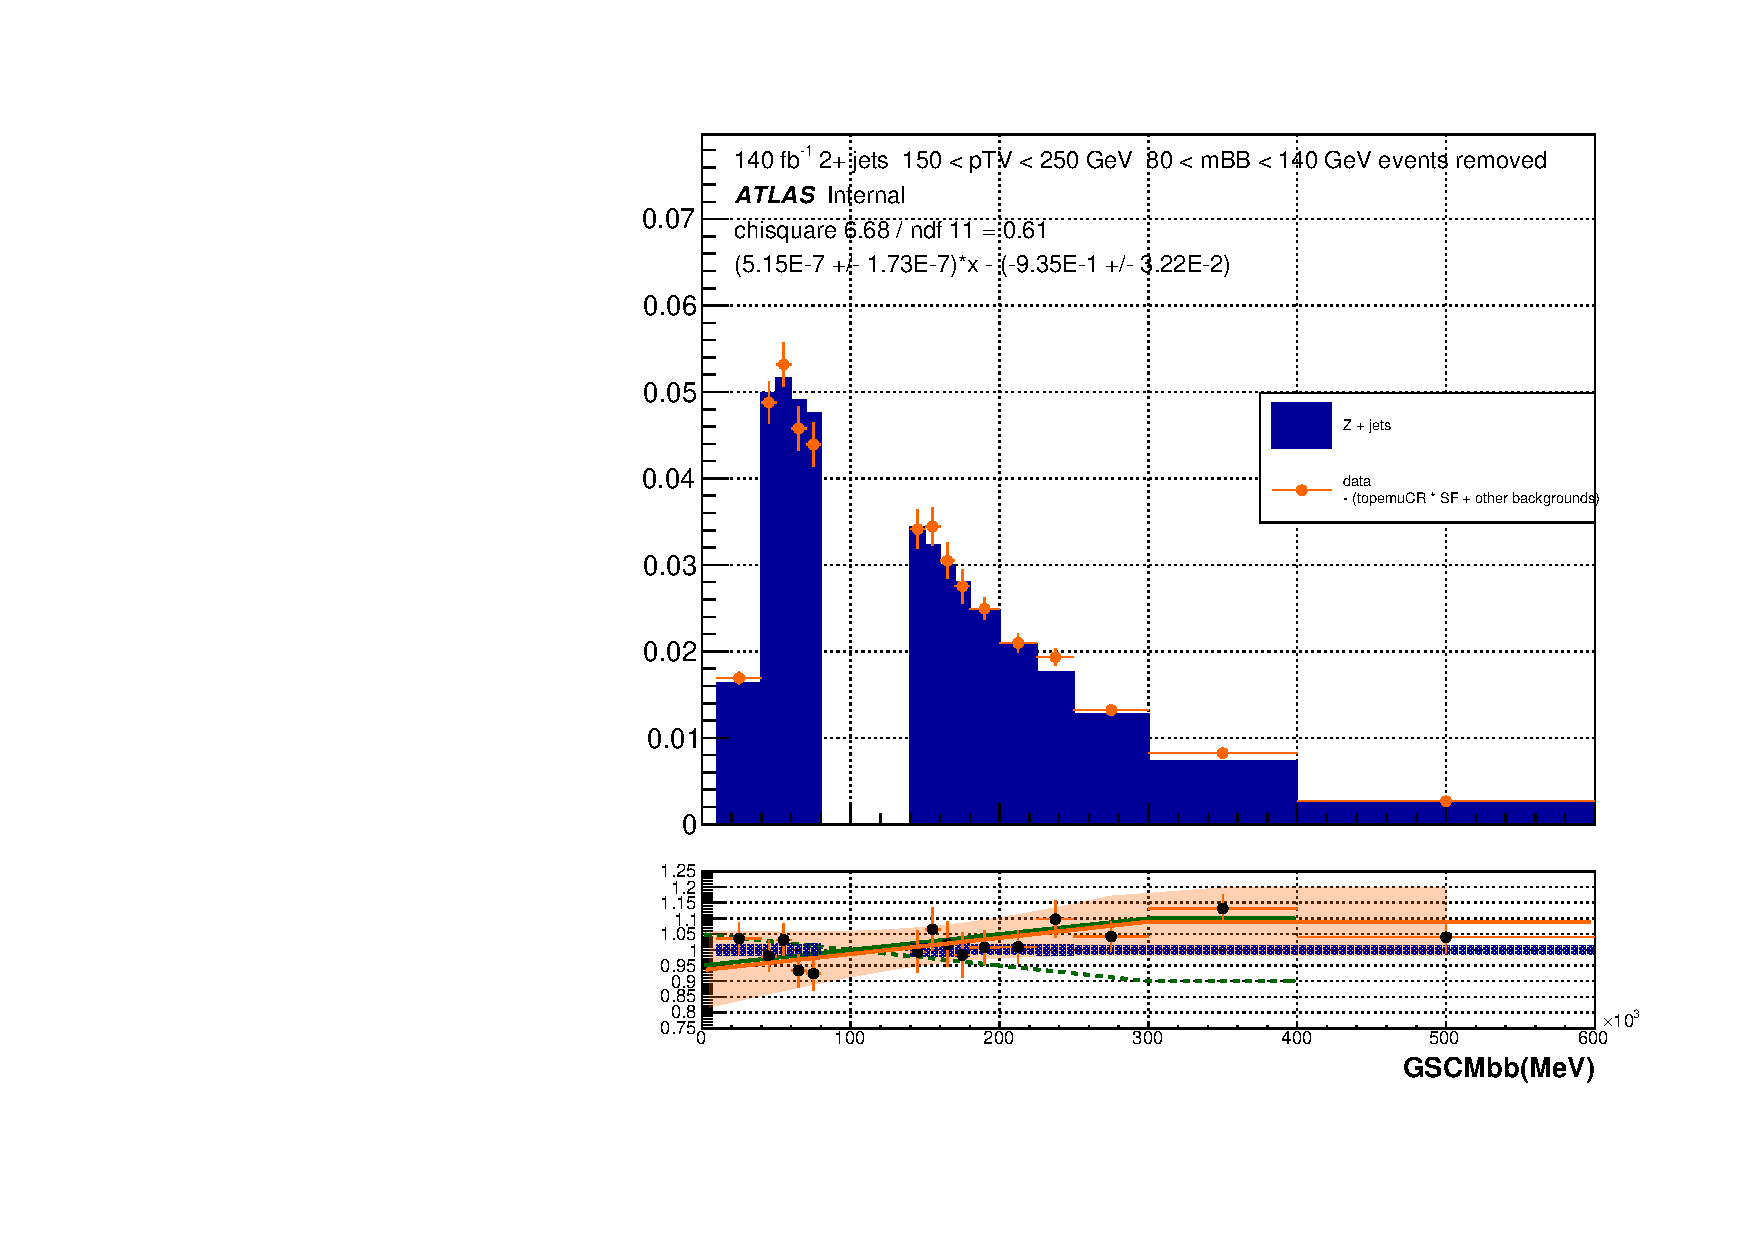
\includegraphics[width=0.49\textwidth]{Zjets-shapes/two_plus_jet_med_blind_ttbardd/two_plus_jet_med_blind_ttbardd_GSCMbb} \\
  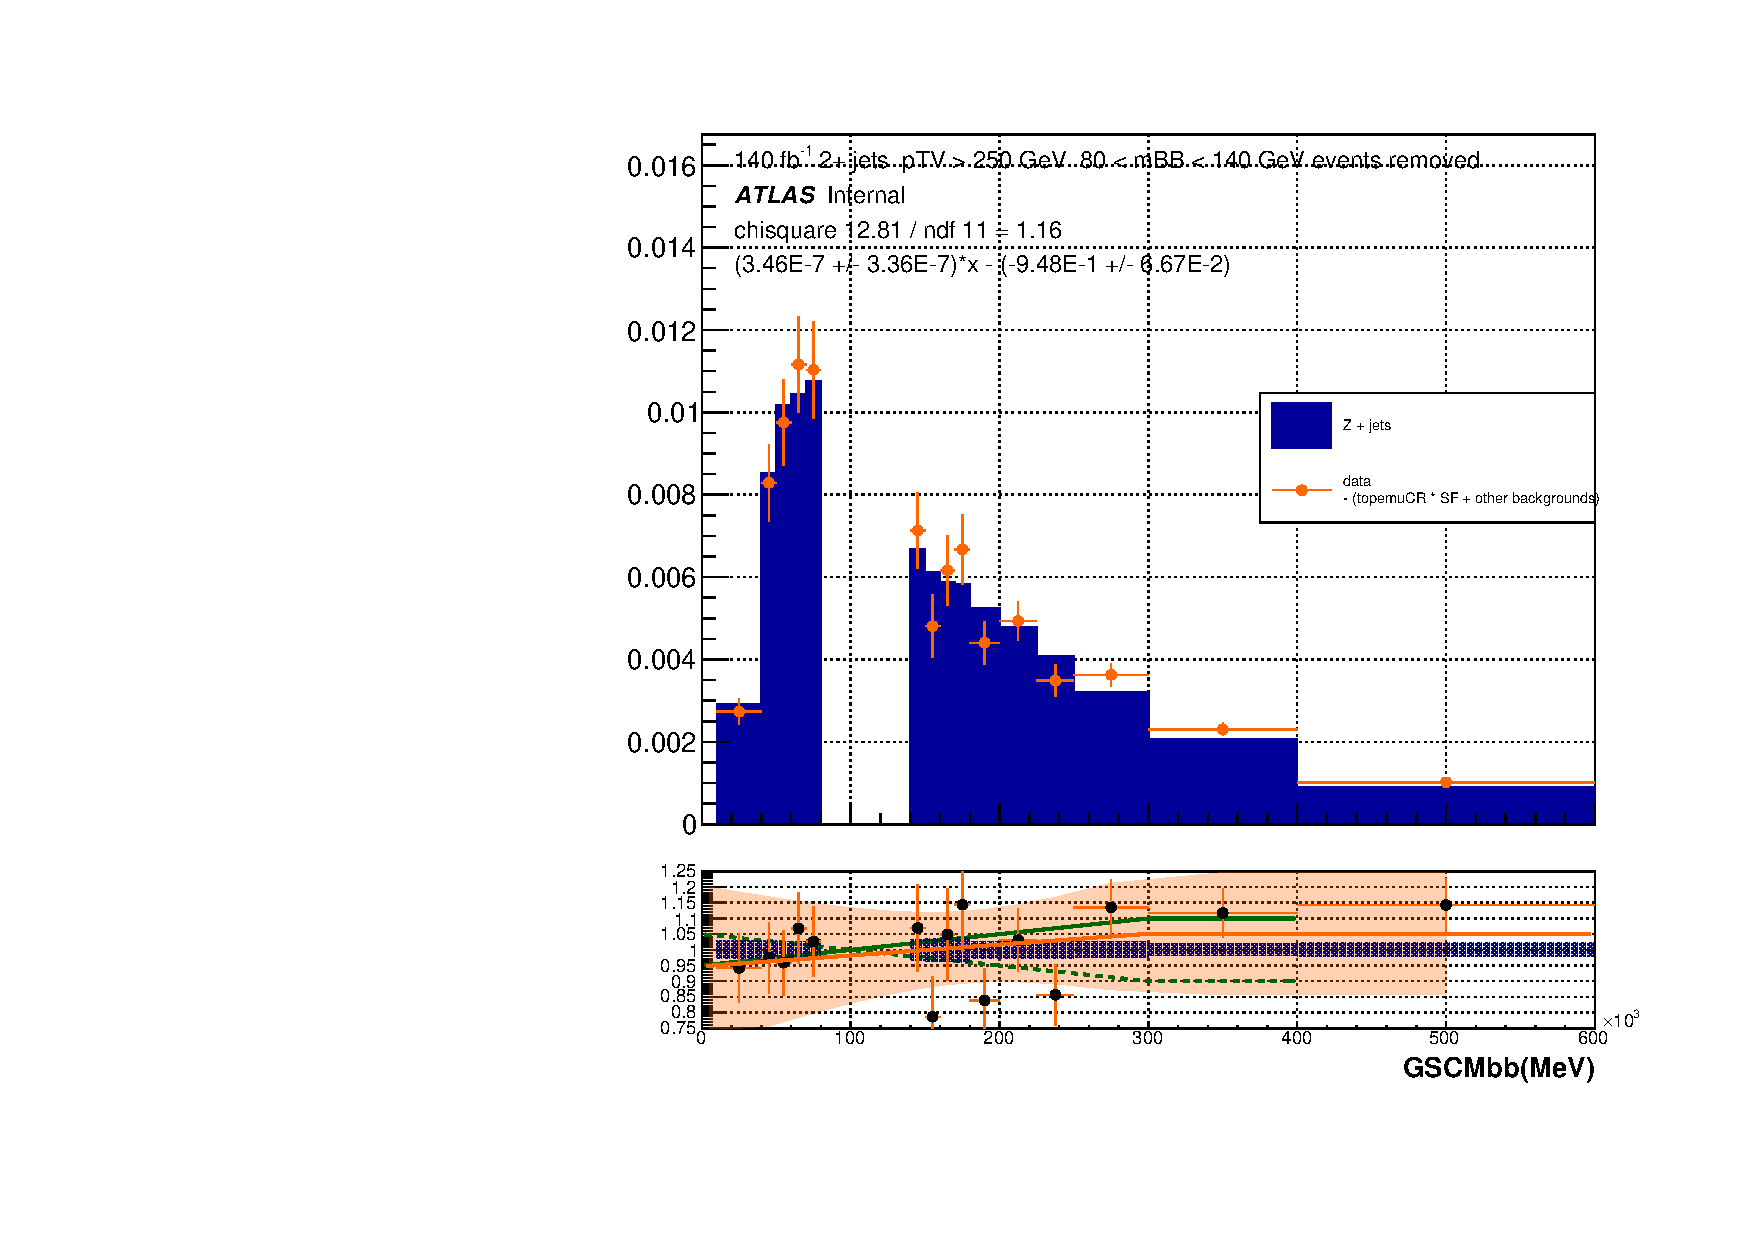
\includegraphics[width=0.49\textwidth]{Zjets-shapes/two_plus_jet_high_blind_ttbardd/two_plus_jet_high_blind_ttbardd_GSCMbb}
  \caption[Subtracted data versus the nominal $Z+$jets prediction, GSC
  $m_{bb}$ across different analysis $p_{\mathrm{T}}^V$ bins.]{Subtracted data
    versus the nominal $Z+$jets prediction in the GSC $m_{bb}$ distribution,
    shown in each of the $p_{\mathrm{T}}^V$ bins of the analysis. The solid and
    dashed green lines in the ratio panel show functional form of the fit used
    in the previous analysis and it's symmetrised version respectively. The
    solid orange line the ratio is the fit to the ratio of the subtracted data
    and the prediction, the shaded region represents the 95~\% confidence
    interval.}
  \label{fig:zjets-mbb-shape-ptv-range}
\end{figure}